\begin{figure}[ht]
 \centering
 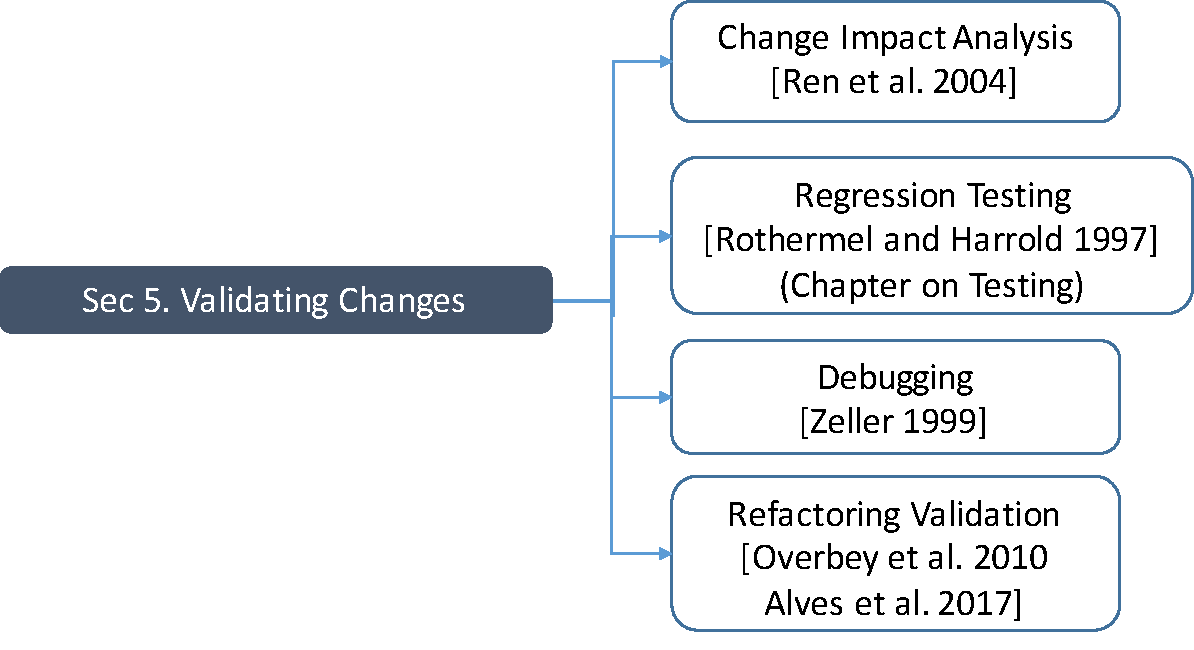
\includegraphics[width=0.6\textwidth]{images/ChangeValidation.pdf} 
 \caption{Change Validation and Related Research Topics} 
 \label{fig:changevalidation} 
\end{figure}

After making software changes, developers must validate the correctness of updated software. Validation and verification is a vast area of research. In this section, we focus on techniques that aim to identify faults introduced due to software changes. As Chapter~\todo{cross reference to testing} discusses the history and seminal work on regression testing in details, we refer the interested readers to that chapter instead. Section~\ref{sec:CIA} discusses Change Impact Analysis, which aims to determine the impact of source code edits on programs under test. Section~\ref{sec:deltadebugging} discusses how to localize program changes responsible for test failures. Section~\ref{sec:refactoringvalidation} discusses the techniques that are specifically designed to validate refactoring edits under the assumption that software's external behavior should not change after refactoring. 

\subsection{Change Impact Analysis} 
\label{sec:CIA} 
Change Impact Analysis onsists of a collection of techniques for determining the effects of source code modifications, and can improve programmer productivity by: (i) allowing programmers to experiment with different edits, observe the code fragments that they affect, and use this information to determine which edit to select and/or how to augment test suites, (ii) reducing the amount of time and effort needed in running regression tests, by determining that some tests are guaranteed not to be affected by a given set of changes, and (iii) reducing the amount of time and effort spent in debugging, by determining a safe approximation of the changes responsible for a given test’s failure. 

In this section, we discuss the seminal change impact analysis work, called Chianti that serve the both purposes of affected test identification and isolation of failure-inducing deltas using a two phase approach in Figure~\ref{fig:twophase}~\cite{Ren2004}: (1) which test cases do I have to rerun on the new version to identify potential regression faults? and (2) for those tests that were selected and failed, which subset of the delta between the two versions led to behavior differences?  

\begin{figure*}
\centering
\begin{minipage}{.45\textwidth}
  \centering
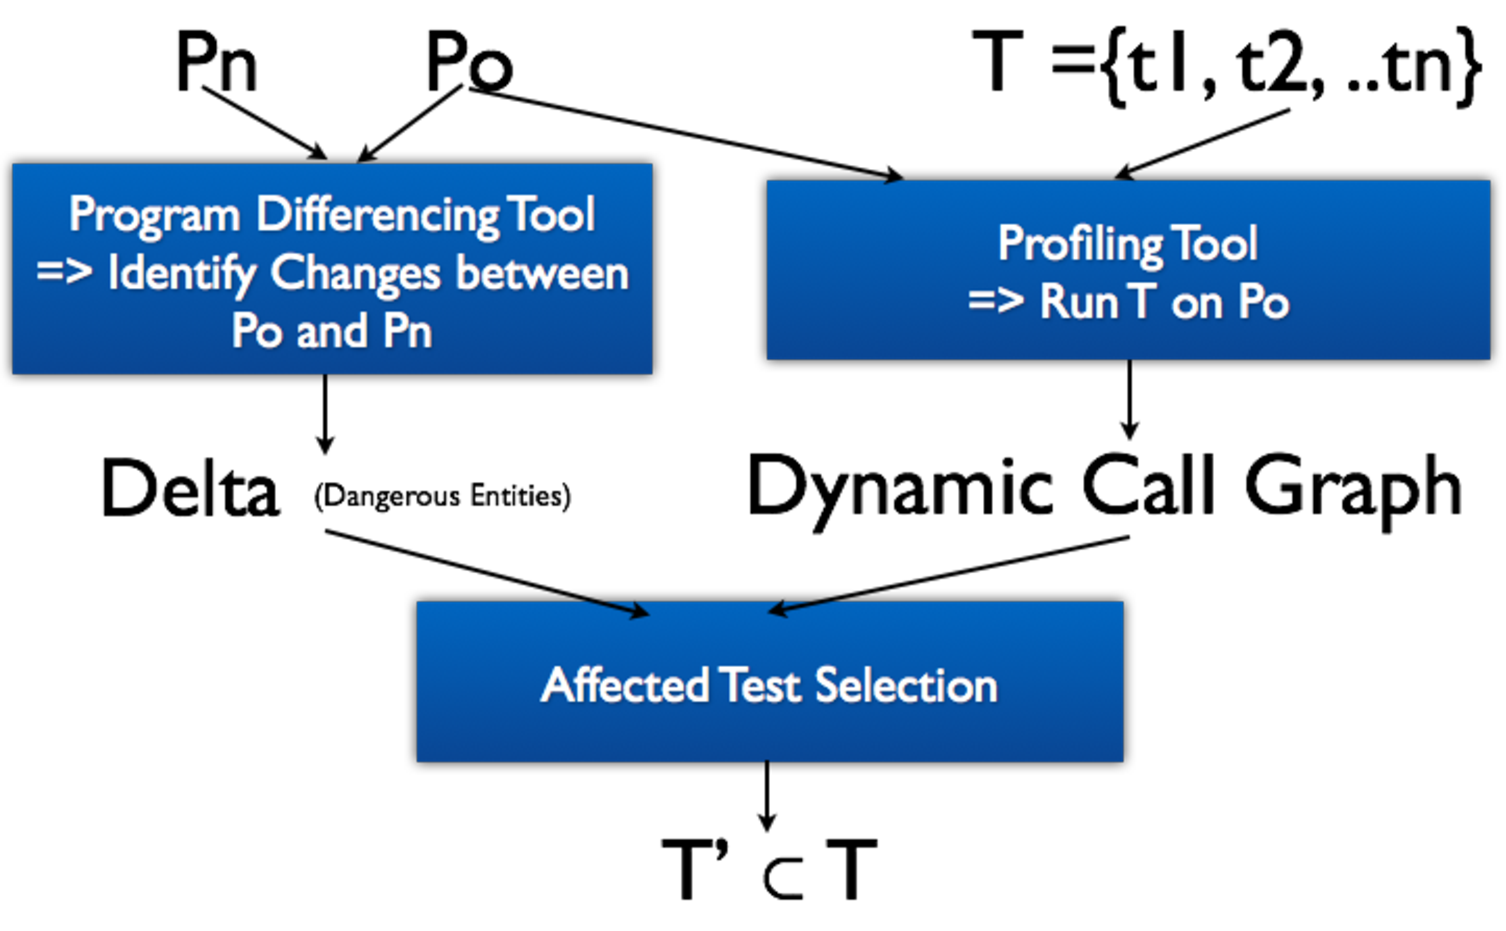
\includegraphics[width=0.9\textwidth]{images/ChiantiPhase1.pdf}
\end{minipage}
\begin{minipage}{.45\textwidth}
  \centering
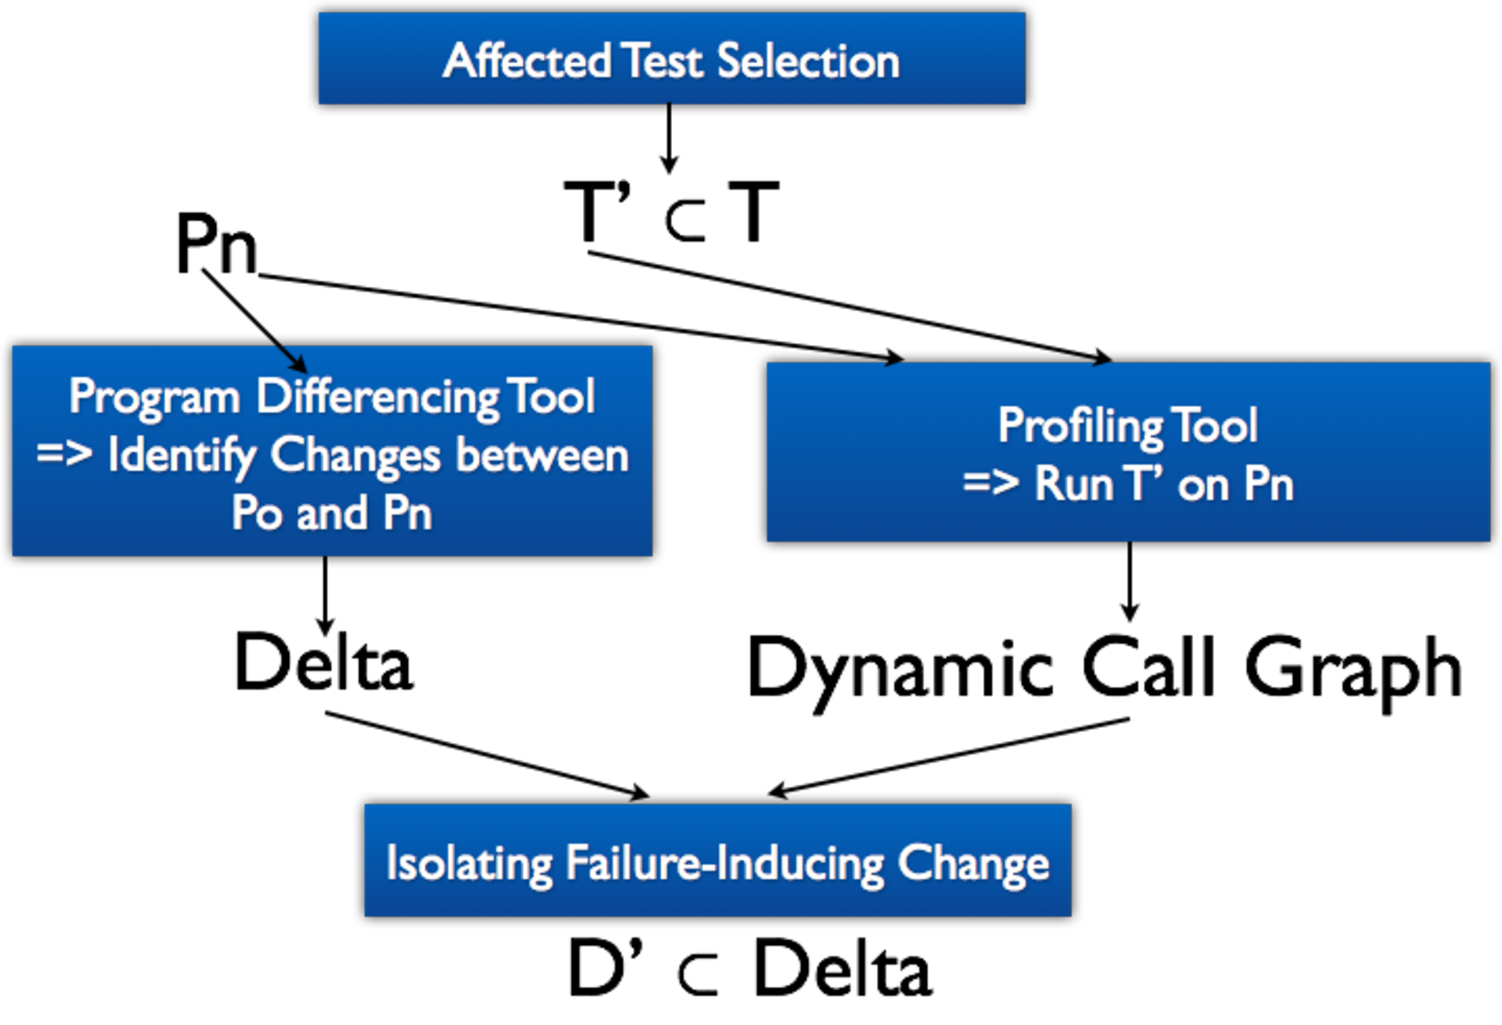
\includegraphics[width=0.9\textwidth]{images/ChiantiPhase2.pdf}
\end{minipage}
\caption{Chianti Change Impact Analysis: identifying affected tests (left) and identifying affecting change (right)} 
\label{fig:twophase} 
\end{figure*}

Chianti constructs dynamic call graphs, modeling programs at a coarser granularity. It compares the syntax tree of the old and new program versions and decomposes the edits into atomic changes at a method and field level. Changes are then categorized as added classes (AC), deleted classes (DC), added methods (AM), deleted methods (DM), changed methods (CM), added fields (AF), deleted fields (DF), and lookup (i.e., dynamic dispatch) changes (LC). For example, Figure~\ref{fig:chianti} shows a software change example and corresponding lists of atomic changes inferred from AST-level comparison. An arrow from an atomic change $A1$ to an atomic change $A2$ indicates that $A2$ is dependent on $A1$. Consider, for example, the addition of the call \codefont{B.bar()} in method \codefont{B.foo()}. This source code change resulted in atomic change \codefont{8}. The LC atomic change category models changes to the dynamic dispatch behavior of instance methods. In particular, an LC change \codefont{LC(Y, X.m())} models the fact that a call to method \codefont{X.m()} on an object of type \codefont{Y} results in the selection of a different method.

Phase I reports {\bf affected tests}\textemdash a subset of regression tests relevant to edits. It identifies a test if its dynamic call graph on the old version contains a node that corresponds to a changed method (CM) or deleted method (DM)  or or if the call graph contains an edge that corresponds to a lookup change (LC). Figure~\ref{fig:chianti} also shows the dynamic call graph of each test for the past version (left) and the current version (right). Using the call graphs on the left, it is easy to see that: (i) \codefont{test1} is not affected, (ii) \codefont{test2} is affected because its call graph contains a node for \codefont{B.foo()}, which corresponds to CM change 8, and (iii) \codefont{test3} is affected because its call graph contains an edge corresponding to a dispatch to method \codefont{A.foo()} on an object of type \codefont{C}, which corresponds to LC change 4.

Phase II then reports {\bf affecting changes}\textemdash a subset of changes relevant to the execution of affected tests in the new version. For example, we can compute the affecting changes for \codefont{test2} as follows. The call graph for \codefont{test2} in the edited version of the program contains methods \codefont{B.foo()} and \codefont{B.bar()}. These nodes correspond to atomic changes 8 and 9, respectively. Atomic change 8 requires atomic change 6, and atomic change 9 requires atomic changes 6 and 7. Therefore, the atomic changes affecting test2 are 6, 7, 8, and 9. Informally, this means that we can automatically determine that \codefont{test2} is affected by the addition of field \codefont{B.y}, the addition of method \codefont{B.bar()}, and the change to method \codefont{B.foo()}, but not on any of the other source code changes. 

\begin{figure*}
\centering
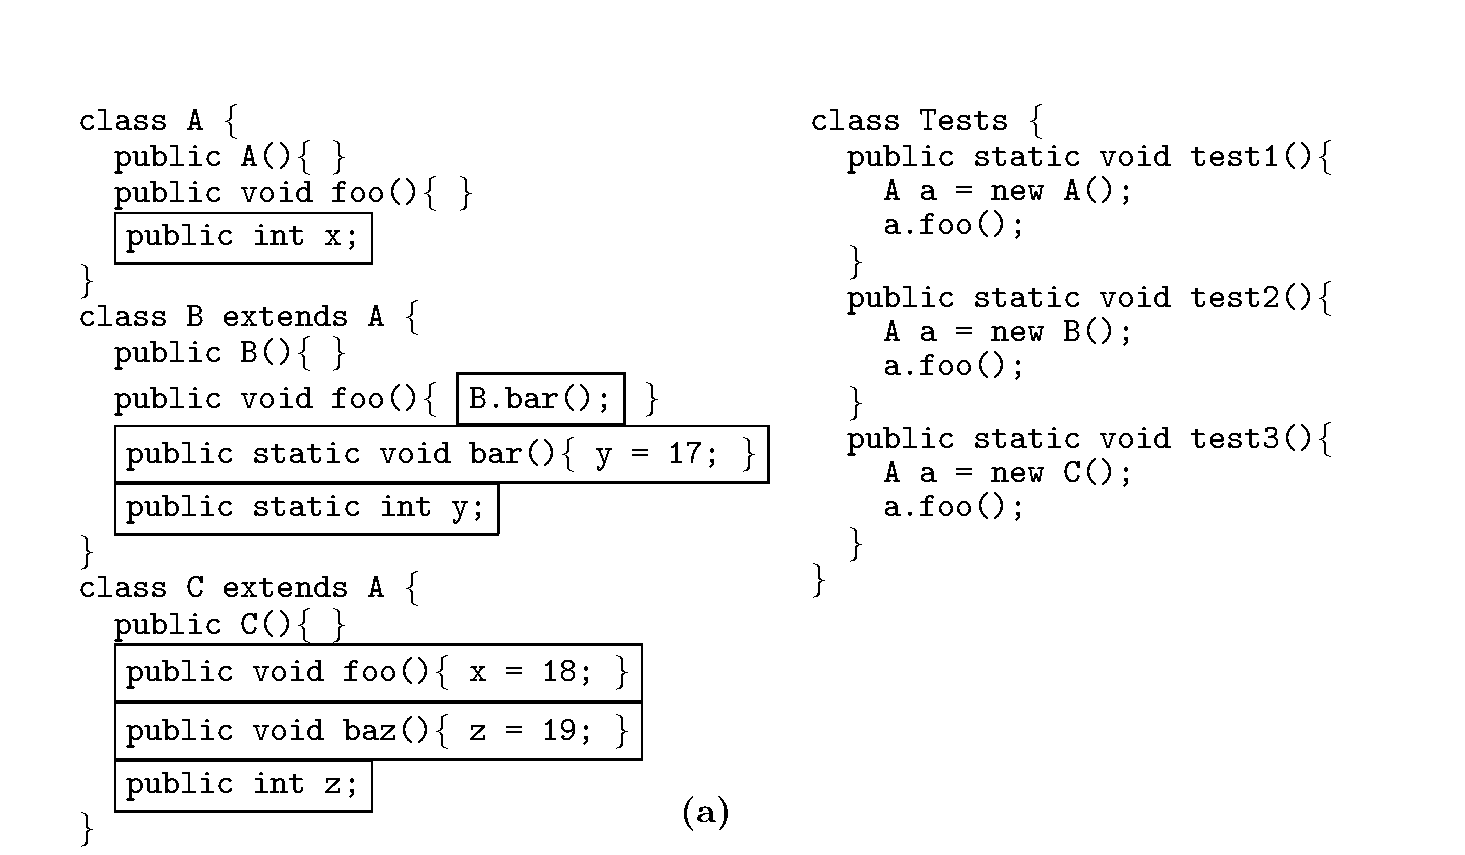
\includegraphics[width=0.95\textwidth]{images/ChiantiExample.pdf}
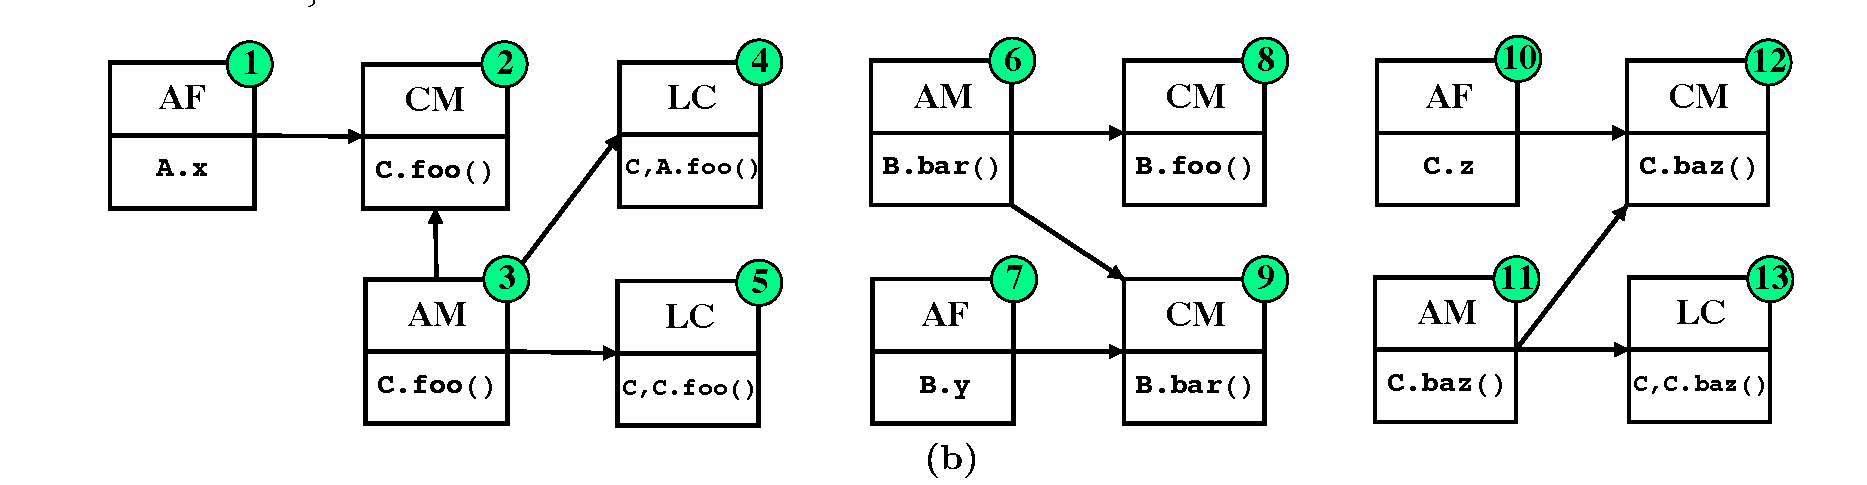
\includegraphics[width=0.95\textwidth]{images/ChiantiAtomicChange.pdf}

\includegraphics[width=0.9\textwidth]{images/DynamicCallGraph.png}
\caption{Chianti change impact analysis} 
\label{fig:chianti} 
\end{figure*}

\subsection{Debugging Changes} 
\label{sec:deltadebugging} 
Delta Debugging~\cite{Zeller1999,zeller01} iteratively applies a subset of all changes to
construct intermediate versions to find a minimum set of changes that lead to
a test failure. However, Delta Debugging considers all changes between
the old and new program version as the candidate set without considering compilation dependences among those changes. Furthermore,
Delta Debugging does not rank these edits according to their test spectra, leaving it to a
programmer to sort out a real culprit of a regression test failure among a
large set of potential failure-inducing changes.

\begin{figure*}
\centering
\begin{minipage}{.48\textwidth}
  \centering
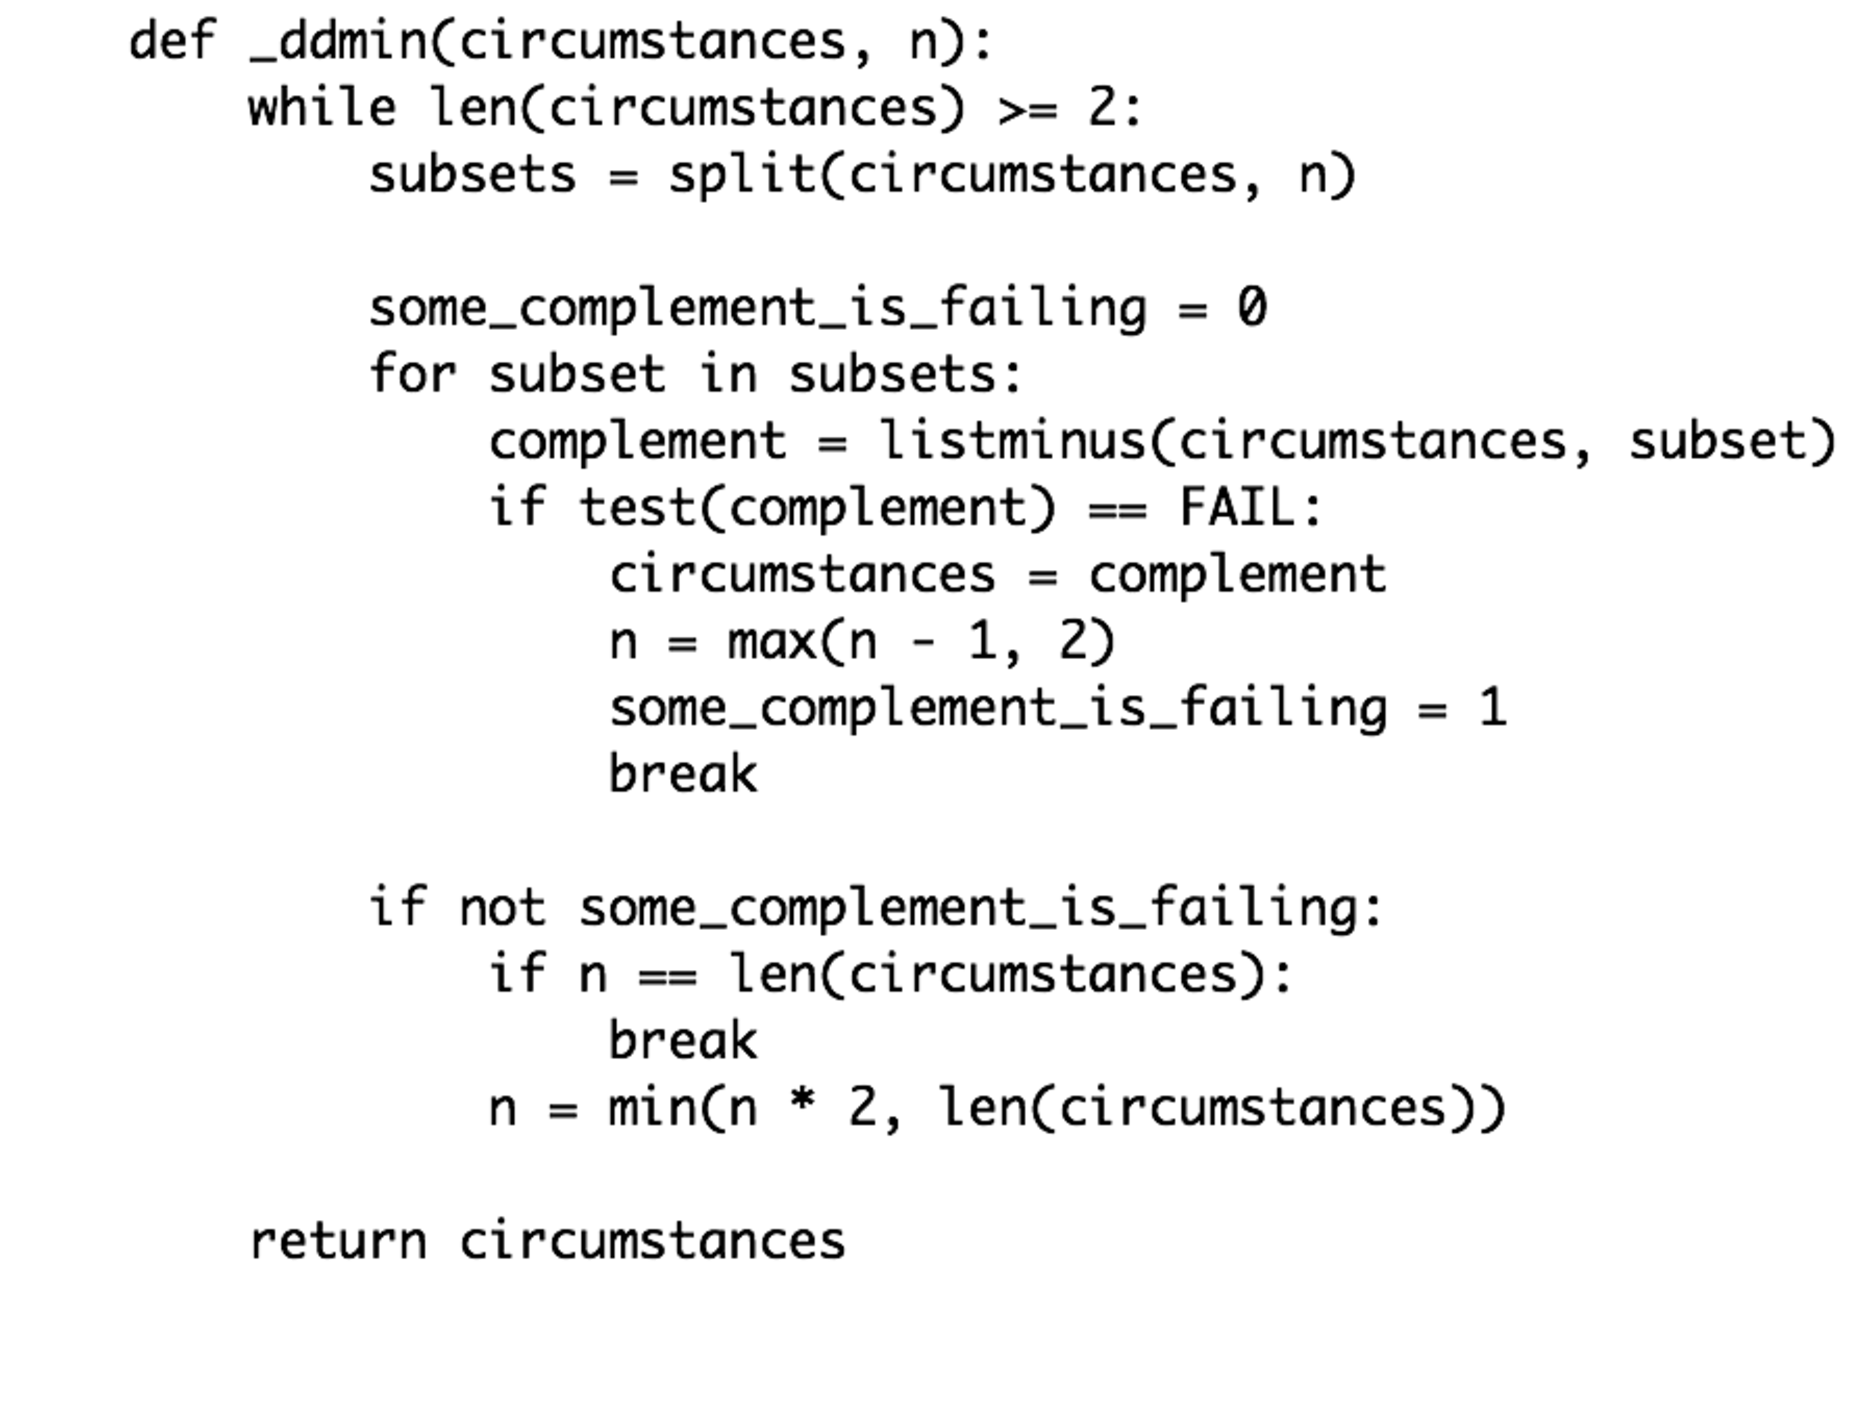
\includegraphics[width=1\textwidth]{images/DeltaDebugging.pdf}
\end{minipage}
\begin{minipage}{.48\textwidth}
  \centering
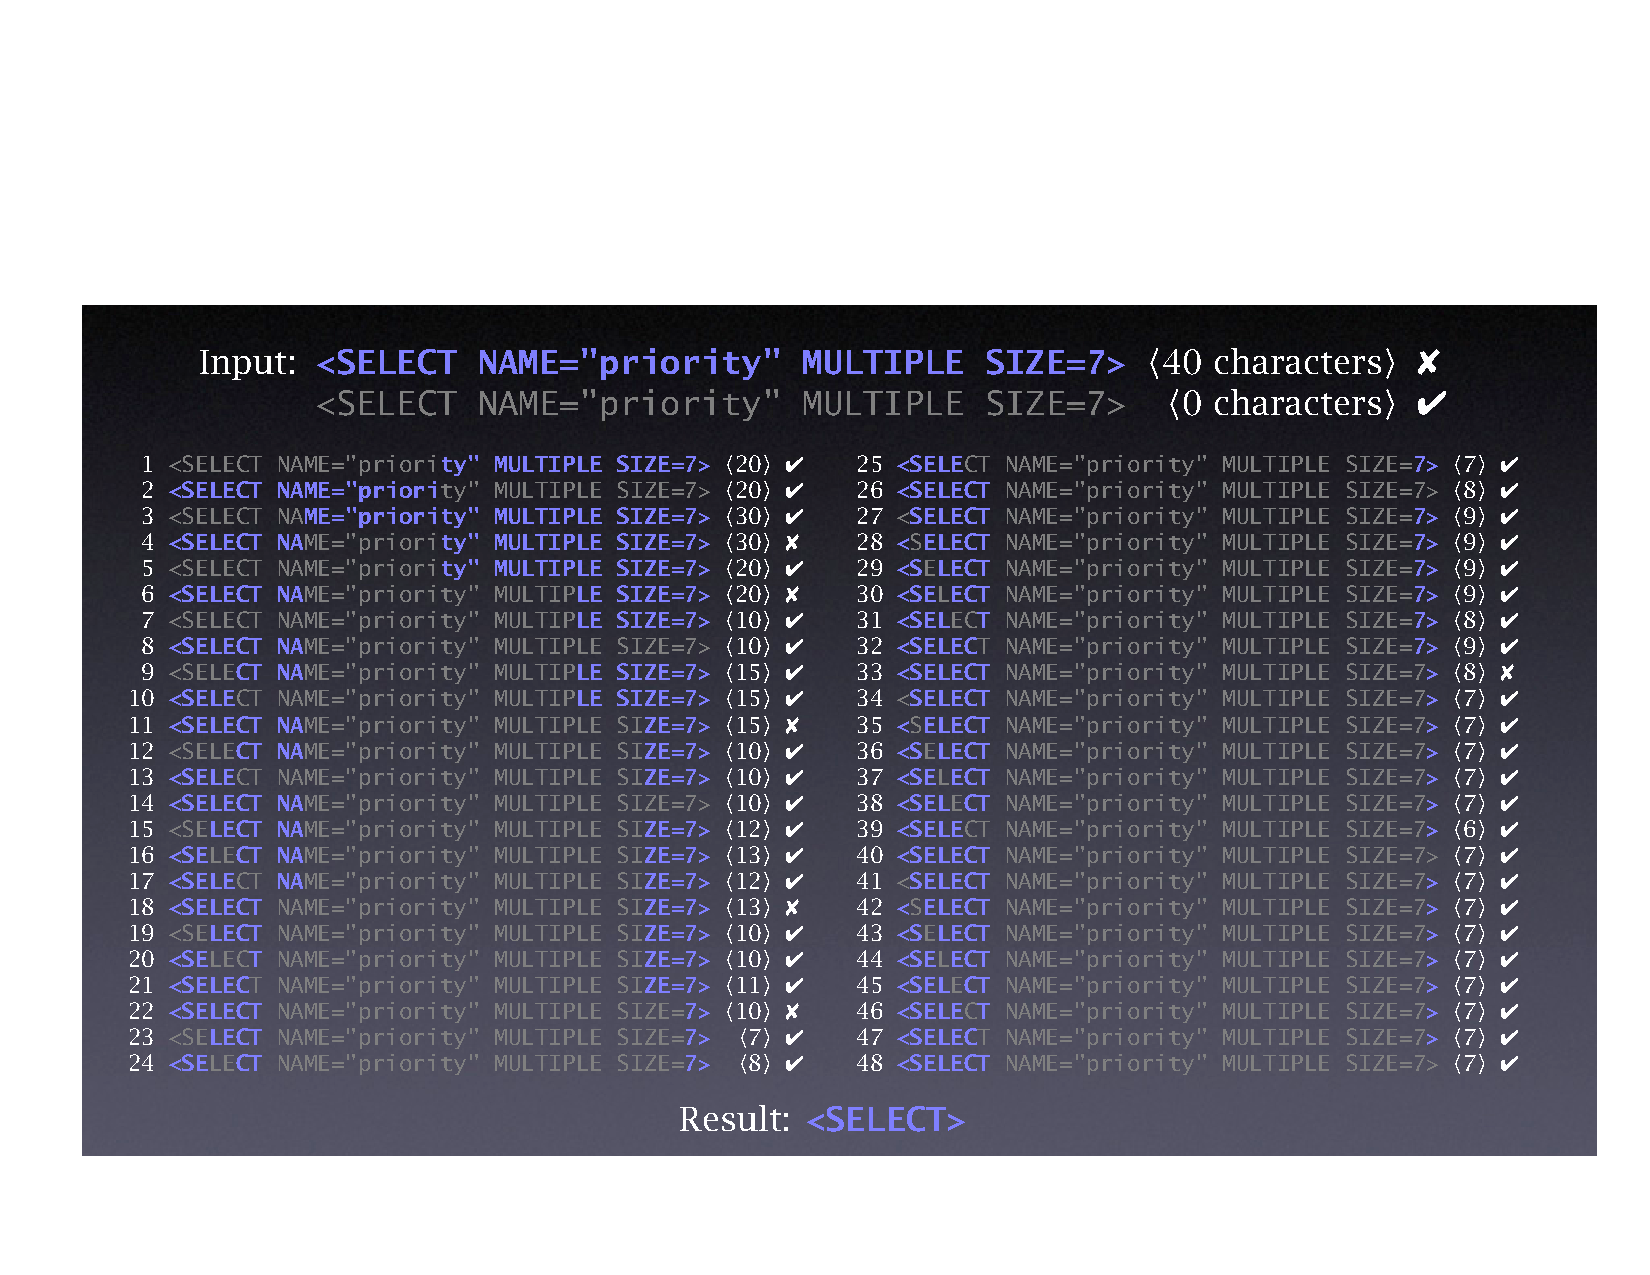
\includegraphics[width=1\textwidth]{images/DeltaDebuggingIlustration.pdf}
\end{minipage}
\caption{Delta Debugging: Algorithm and Illustration} 
\label{fig:deltadebugging} 
\end{figure*}


Spectrum-based fault localization techniques~\cite{hao2005similarity,Hao:com09,harrold05tarantula,Abreu:testing07,Baudry:icse06,liblit05,Yanbing:icse08, abreu2009practical} such as Tarantula~\cite{Jones2002:tarantula} statistically compute suspiciousness scores for statements based on execution traces of both passed and failed test cases, and rank potential faulty statements based on the derived suspiciousness scores. Recently, researchers have also introduced more suspiciousness computation measures to the realm of fault localization for localizing faulty statements~\cite{naish2011model, lo2010comprehensive}. For example, Lucia et al.~\cite{lo2010comprehensive} introduced 20 association measures to the area of spectrum-based fault localization and compare them against Tarantula~\cite{Jones2002:tarantula} and Ochiai~\cite{Abreu:testing07}. Researchers have also developed various automated tool-sets which embodies different spectrum-based fault localization techniques~\cite{tarantula-url, janssen2009zoltar}. However, such spectrum-based fault localization techniques are not scalable to large evolving software systems, as they compute spectra on all statements in each program version and do not leverage information about program edits between the old and new versions.

FaultTracer~\cite{zhang2011localizing}, combines the strengths of Chianti-style change impact analysis and Tarantula-style fault localization. To present a ranked list of potential failure-inducing edits, FaultTracer applies a set of spectrum-based ranking techniques to the affecting changes determined by Chianti-style change impact analysis. It uses a new enhanced call graph representation to measure test spectrum information directly for field-level edits and to improve upon the existing Chianti algorithm. Ren et al.~\cite{Ren2007} propose a heuristic ranking algorithm for method-level edits based on their numbers of ancestors, descendants, callers and callees on call graphs of tests. Ren et al.'s heuristic is confined to rank only method-level edits, while FaultTracer uses test profile at the level of {\em extended call graphs} to consider both method calls and field accesses and can rank all types of program edits including addition, modification, and deletion of methods, as well as fields.  

\subsection{Refactoring Validation} 
\label{sec:refactoringvalidation} 

Schaeffer et al.~validate refactoring edits by comparing data and control dependences between two program versions~\cite{Schaefer2010:refactoring}. As opposed to validating refactoring edits, Daniel et al. focus on testing refactoring engines by systematically generating input programs for refactoring transformations~\cite{Brett2007:reftest}. 

Regression testing is the most used strategy for checking refactoring correctness. However, Rachatasumrit and Kim~\cite{Rachatasumrit2012:refactortest} find that test suites are often inadequate and developers may hesitate to initiate or perform refactoring tasks due to inadequate test coverage~\cite{Kim2012:FSR}. Soares et al.~\cite{Soares:icse10} design and implement SafeRefactor that uses randomly generated test suites for detecting refactoring anomalies. Mongiovi et al.~\cite{mongiovi2013making} introduces SafeRefactorImpact. SafeRefactorImpact extends SafeRefactor by adding an impact analysis step. SafeRefactorImpact decomposes an edit into small-grained transformations and analyzes the impact of each one. Then, it uses Randoop to generate test cases for the impacted methods. In our studies, we show that even tool-generated tests can be inadequate. Using a SafeRefactor like testing validation, we find that about 25\% of the refactoring anomalies are not identified by using generated test suites, even with a long generation time limit (100 seconds). 

Formal verification is an alternative for avoiding refactoring anomalies~\cite{Mens2004:SSR}. Corn\'elio et al.~\cite{cornelio2010sound} propose rules for guaranteeing semantic preservation. Similarly, Mens et al.~\cite{mens2005formalizing} use graph rewriting for specifying refactorings. Overbey et al.~\cite{overbey2010collection} present a collection of refactoring specifications for Fortran 95. However, these approaches focus on improving the correctness of automated refactoring through formal specifications, as opposed to finding anomalies during manual refactoring. 


RefDistiller is a static analysis approach~\cite{Alves2017:refdistiller,Alves:2014:RRA:2635868.2661674} to support the inspection of manual refactorings. It combines two techniques. First, it applies predefined templates to identify potential missed edits during manual refactoring. Second, it leverages an automated refactoring engine to identify extra edits that might be incorrect, helping to  determine the root cause of detected refactoring anomalies.

GhostFactor~\cite{geManual2014} checks the correctness of manual refactoring, similar to RefDistiller. 
However, unlike RefDistiller, GhostFactor does not have any capability to isolate potential behavior changes from pure refactoring by running an equivalent automated refactoring. GhostFactor detects missing edits only, while RefDistiller detects both missing and extra edits. 

Ge and Murphy-Hill~\cite{emersoncodereview:2014chase} propose a refactoring-aware code review tool, with goals similar to RefDistiller. This tool helps reviewers by identifying applied refactorings and letting developers examine them in isolation. Ge and Murphy-Hill leverage Eclipse refactoring APIs to separate pure refactorings. RefDistiller goes a step further by extending Eclipse refactoring APIs to prevent unsafe refactoring by checking bug conditions, allowing to apply automated refactoring in a safe manner when isolating pure refactoring. 


Other approaches ensure the consistency between refactored programs and other software artifacts like design models~\cite{Bottoni2003:coordinatedTransformation,Straeten2003:UML}. For example, Bottoni et al.~modeled a refactoring as a set of distributed graph transformations~\cite{Bottoni2003:coordinatedTransformation}. Each time a code refactoring is applied, the corresponding graph transformations are automatically applied to related design models to preserve consistency. Van Der Straeten et al.~suggested using description logic to maintain the consistency between relevant UML models as they evolve~\cite{Straeten2003:UML}.


